\documentclass[12pt,fleqn]{article}\usepackage{../../common}
\begin{document}
Lineer Programlama ve Simplex

LP, Operasyonel Araştırma konusunun mihenk taşlarından biridir, ve bu alanda
George Dantzig simplex buluşu ile lineer optimizasyon alanında çığır açmıştır.
Lineer programlama ile çözülebilen problemlerde bir hedef fonksiyonu vardır, tüm
değişkenler artı değerdedir, ve sınırlama (constraint) ifadeleri vardır, bu
ifadeler $a_1x_1 + a_2x_2 + ... + a_nx_n \le b$ şeklinde olurlar, ki $b > 0$
olacak şekilde.

Örnek

6000 akrelik (1 akre 0.4 hektara eşdeğer) bir tarlada ya mısır ya da soya
ekebiliriz. Mısırın her akresi için 9 galon (1 galon 3.78 litre) gübre, ve 3/4
saatlik işçilik gerekli. Her akre soya için 3 galon gübre ve 1 saat işçilik
gerekli. Çiftçinin elinde 40500 galonluk gübre, ve en fazla 5250 saatlik iş gücü
var. Eğer mısır için galon başına 60 lira, soya için 40 lira para kazanılıyorsa,
tarlada ne kadar mısır ve soya ekilmelidir ki kazanç maksimize edilsin [3,
  sf. 306]?

Eğer $x$ mısır $y$ soya miktarı ise, 

$$ \textrm{maksimize et  } 60x + 40y, \textrm{ öyle ki} $$ 
$$ x + y \le 6000 $$
$$ 9x + 3y \le 40500 $$
$$ \frac{3}{4}x + y \le 5250 $$ 

Daha fazla ilerlemeden önce bazı numaralar: bugünlerde bu tür problemler
bilgisayar üzerinden çözülüyor, ve her çözüm paketi girdileri farklı
şekilde isteyebilir. Kimisi maksimizasyon değil minimizasyon çözmek için
yazılmıştır mesela. Dert değil, bir maksimizasyon problemini minimizasyona
çevirmek için hedef fonksiyonunu eksi ile çarpmak yeterli (ya da
minimizasyonu maksimizasyon yapmak için, ters yönde). O zaman $-60x - 40y$
ifadesini minimize de edebilirdik.

Pay bırakma değişkenleri (slack variables): Küçüktür büyüktür işaretlerini
eşitlik ifadelerine çevirmek istiyorsak, bunun için pay bırakma / gevşeklik
değişkenleri kullanabiliriz. Mesela

$$ x + y \le 6000 $$

ifadesini

$$ x + y + s_1 = 6000 $$

olacak şekilde değiştirebiliriz, ki $s_1 \ge 0$. Pay bırakma kelimesinin nereden
geldiğini görebiliyoruz burada, sanki $s_1$, $x+y$ değeri ve 6000 değeri
arasında bir ``pay bırakıyor'', bir gevşeklik olmasını sağlıyor. Eğer $x+y$ en
fazla 6000 olabilirse o zaman $x+y$ ile 6000 arasındaki fark kadar bir bölgede
bir başka değişken tanımlanabilir, ve bu değişkenin herhangi bir değere sahip
olmasına izin verilir, yeter ki $x+y+s_1$ 6000'e eşit olsun.

Küçüktür ya da eşittir ifadelerini böyle çevirebiliriz. Büyüktür ya da eşittir
ifadeleri için,

$$ x + y \ge c $$

$$ -x - y \le -c $$

$$ -x - y + s_1 = -c $$

$$ x + y - s_1 = c $$

Yani büyüklük ifadelerini negatif pay bırakma değişkenleri ile eşitliğe
çevirebiliriz. Aynı şekilde diğer eşitsizlikleri değiştiririz, tabii her değişim
için ayrı bir pay bırakma değişkeni gerekir, $s_2,s_3,..$ böyle devam eder.

Hedef fonksiyonu da ufak bir değişim üzerinden aynı sınırlamalar listesine dahil
edilebilir, $P = 60x + 40y$ hedefi $-60x -40y + P = 0$ olarak değiştirilir.

Tüm denklem sistemi şöyle,

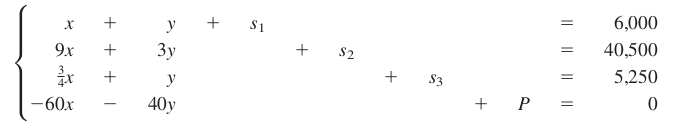
\includegraphics[height=2.5cm]{func_simplex_01.png}

Bu sistemi matris üzerinden göstermek daha kolay,

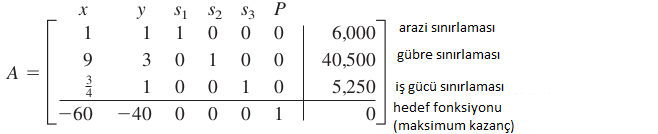
\includegraphics[height=3cm]{func_simplex_02.png}

Çözümün genel stratejisi şudur: matris üzerinde satır bazlı değişim yaparak (ki
bu tür değişimlerin lineer denklem sisteminde değişiklik yaratmadığını
biliyoruz) matrisin $x,y$ değişkenlerinin olduğu bölgede sadece $1,0$
değerleri kalacak hale getir. Ardından $x,y$ çözümünü matrisin en sağ kolonundan
oku.

Değişimleri yaparken tabii ki maksimizasyon amacına en hızlı erişecek şekilde bu
değişimleri yapmak isteriz.

En son satır hedef fonksiyonuna tekabül ediyor, ve amacımız maksimizasyon olduğu
için, maksimizasyona en hızlı şekilde erişmenin en iyi yolu en son satırda
değeri en küçük (en negatif) olan değeri değiştirmek. Bu kolonu pivot kolonu
olarak seçeriz.

Bu kolondaki hangi öğeyi seçeceğiz? Onun için o kolondaki her ögeyi matrisin en
sağındaki kolonda ona tekabül eden öğeye bölerek sonuca bakarız. Bu sonuçların
içinde hangisi daha küçük ise o hücre pivot ögesi haline gelir. Bu seçim, ve
sebepleri hakkında daha teorik detaylar [6, sf. 382]'da bulunabilir.

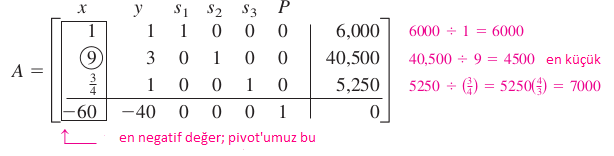
\includegraphics[height=3cm]{func_simplex_03.png}

Pivot ögesi 9'u 1 haline getirmek ve o kolonda diğer tüm değerleri sıfırlamak
için satır operasyonları yaparız ($R_i$ i'inci satır anlamında).

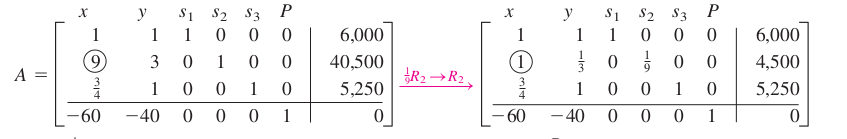
\includegraphics[height=2.5cm]{func_simplex_04.png}

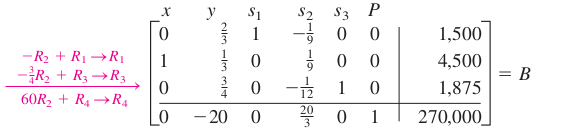
\includegraphics[height=2.5cm]{func_simplex_05.png}

Bu şekilde $A$ matrisini $B$'ye dönüştürdük. Şimdi aynı algoritmaya devam
edelim. En negatif değer hangisi? -20 değeri,

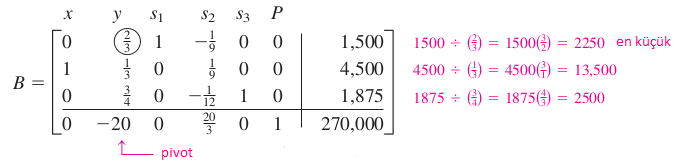
\includegraphics[height=3cm]{func_simplex_06.png}

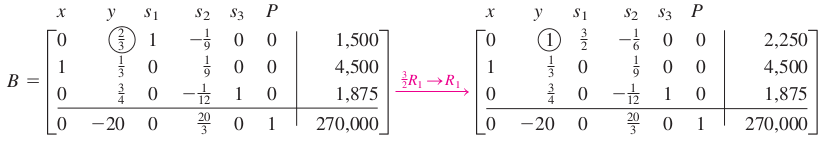
\includegraphics[height=2.8cm]{func_simplex_07.png}

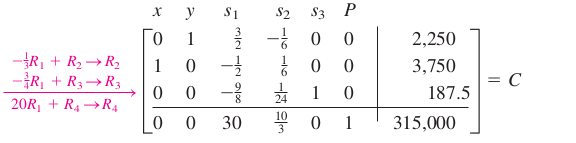
\includegraphics[height=2.8cm]{func_simplex_08.png}

Böylece $C$ matrisine eriştik. Amaçladığımız gibi $x,y$ bölgesinde 1 ve 0
değerleri var, bu noktada hedef fonksiyonun optimal değeri 315,000 (sağ alt
köşe), ve $y=2250, x=3750$ bu optimal değer anındaki $x,y$ değerleri. Demek ki
çiftçinin tarlasının 3750 akresinde mısır, 2250 akresinde soya ekmesi onun için
en kazançlısı olacak.

Algoritma en alt satırda hiç negatif değer kalmayıncaya kadar devam eder. 

Not: Her problem üstteki gibi acısız çözülemeyebilir; birden fazla, ya da hiç
çözüm olmadığı durumlar vardır, bu gibi farklı şartlar için [3]'e
danışılabilir. En iyisi tabii ki tüm bu hesapları ve şartları gözönüne alabilen
bir optimizasyon yazılımını kullanmak. Altta bunun örneğini göreceğiz.

Berlin'e Hava İkmali (Berlin Airlift)

Simplex, 2. Dünya Savaşı sırasında Berlin'e Hava İkmali adlı yardım
operasyonunda yoğun bir şekilde kullanıldı. 24 Haziran 1948'te Sovyetler Birliği
Doğu Almanya'dan Berlin'e giden tüm kara ve deniz yollarını tıkadı. Bu yüzden
Berlin'de yaşayan 2 milyon insana yiyecek, giyim, vb. eşyaları nakil edebilmek
için Amerikalı ve İngiliz uçaklarından oluşan dev bir nakliyat operasyonu
planlandı. Elde sınırlı miktarda uçak, kargo kapasitesi vardı ve diğer bazı
kısıtlamalar (constraints) da göz önüne alınarak, durum bir lineer programa
verildi ve optimal seferler planlandı. Simplex metodunun muciti George Dantzig
bu problem üzerinde bizzat uğraştı.

Bu problemin tam tanımı halen yayınlanmış değil, fakat esasına en yakın olan bir
örnek [5, sf. 20]'de bulunabilir. Bir diğeri, [4] baz alınarak, şöyle:
Değişkenler 3 tip uçağın kaç tanesinin yiyecek ve kömür için kullanılacağı, yani
6 değişken var, bunlar 1. tip uçak yiyecek için $x_{1f}$, kömür için $x_{1c}$
diye gidiyor, diğerleri $x_{2f}$, $x_{2c}$, $x_{3f}$, $x_{3c}$.

Kısıtlamalar şöyle; 1500 tondan daha fazla yiyecek, 3500 tondan daha fazla kömür
lazım. 1. tip uçaktan en fazla 10 tane kullanabiliriz, 2. tipten en fazla 22
tane, 3. tipten 10 tane. 

Hedef fonksiyonu bir minimizasyon, bir masraf fonksiyonu bu, yani en az masrafı
olacak şekilde hedefe ulaşmak istiyoruz, hepsini bir arada gösterelim,

$$ \textrm{minimize et  }
1000 x_{1f} + 1000 x_{1c} + 2000 x_{2f} + 2000 x_{2c} + 1200 x_{3f} + 1200 x_{3c},
\textrm{ öyle ki} $$ 
$$ 100 x_{1f} + 200 x_{2f} + 150 x_{3f} \ge 1500$$
$$ 100 x_{1c} + 200 x_{2c} + 150 x_{3c} \ge 3500 $$
$$ x_{1f} + x_{1c} \le 10 $$
$$ x_{2f} + x_{2c} \le 22 $$
$$ x_{3f} + x_{3c} \le 10 $$

Basitleştirme amaçlı olarak $x_{1f},x_{1c},..$ yerine $x_1,x_2,..$ kullanalım,
yani düz sayı bazlı indisler olsun.

Bu problemde hem daha küçüktür, hem daha büyüktür türünden eşitsizliklerin
karışık şekilde kullanıldığını görüyoruz. Eşitsizliklerin hepsini pay bırakma
değişkenleri üzerinden eşitliklere çevireceğimiz için bu dert değil.

Bu problemi çözerken \verb!scipy.optimize! adlı bir kütüphane çağrısı
kullanacağız. Bu çağrı minimizasyon yapar (yani maksimizasyon problemlerinin
hedefi eksi ile çarpılarak tersine çevirilmelidir) ve girdi olarak hem
eşitsizlik, hem eşitlik şartlarını alabilir, biz \verb!A_eq!, \verb!b_eq!
parametreleri üzerinden ikincisini kullanacağız.

\begin{minted}[fontsize=\footnotesize]{python}
from scipy.optimize import linprog
import numpy as np

A = np.array([[-100.,0,-200.,0,-150.,0.,-1.,0,0,0,0],
              [0,-100.,0,-200.,0,-150.,0,-1.,0,0,0],
              [1.,1.,0,0,0,0,0,0,1.,0,0],
              [0,0,1.,1.,0,0,0,0,0,1.,0],
              [0,0,0,0,1.,1.,0,0,0,0,1.]])

b = np.array([-1500., -3500., 10., 22., 10.])

c = np.array([1000., 1000., 2000., 2000., 1200., 1200.,0,0,0,0,0])

res = linprog(-c, A_eq=A, b_eq=b, options={"disp": True})

print (res)
\end{minted}

\begin{verbatim}
Optimization terminated successfully.
         Current function value: -50000.000000
         Iterations: 7
     fun: -50000.0
 message: 'Optimization terminated successfully.'
     nit: 7
   slack: array([], dtype=float64)
  status: 0
 success: True
       x: array([  0. ,  10. ,   7.5,  12.5,   0. ,   0. ,   0. ,
                   0. ,   0. , 2. ,  10. ])
\end{verbatim}

Sonuç ilginç, 3. tip uçaktan hiç seçim yapılmamış. Bu mantıklı aslında çünkü
3. tip uçağın işletim masrafı 1.'den daha fazla ve bu uçaklardan elimizde 1. tip
kadar var.

Bir numara: pay bırakma değişkenlerinin ana matris içinde sadece köşegen
üzerinde değerlerinin olduğu dikkati çekmiş olabilir. Bu matrisi daha hızlı bir
şekilde, ayrı yaratıp soldaki diğer kısma eklesek kodlama daha hızlı olmaz mı?
Evet; pay bırakma değişkenlerini bir vektörde tutup bir birim matrisi ile
çarparsak

\begin{minted}[fontsize=\footnotesize]{python}
svec = [-1,-1,1,1,1]
print np.eye(5,5) * svec
\end{minted}

\begin{verbatim}
[[-1. -0.  0.  0.  0.]
 [-0. -1.  0.  0.  0.]
 [-0. -0.  1.  0.  0.]
 [-0. -0.  0.  1.  0.]
 [-0. -0.  0.  0.  1.]]
\end{verbatim}

sağdaki kısmı elde ederiz. Şimdi soldaki kısma \verb!hstack! ile ``yapıştıralım'',

\begin{minted}[fontsize=\footnotesize]{python}
A = np.array([[-100.,0,-200.,0,-150.,0.],
              [0,-100.,0,-200.,0,-150.],
              [1.,1.,0,0,0,0],
              [0,0,1.,1.,0,0],
              [0,0,0,0,1.,1.]])

print np.hstack((A, np.eye(5,5)*svec)) 
\end{minted}
	      
\begin{verbatim}
[[-100.    0. -200.    0. -150.    0.   -1.   -0.    0.    0.    0.]
 [   0. -100.    0. -200.    0. -150.   -0.   -1.    0.    0.    0.]
 [   1.    1.    0.    0.    0.    0.   -0.   -0.    1.    0.    0.]
 [   0.    0.    1.    1.    0.    0.   -0.   -0.    0.    1.    0.]
 [   0.    0.    0.    0.    1.    1.   -0.   -0.    0.    0.    1.]]
\end{verbatim}

İkmal Problemi, Tekrar

Bu ikmal probleminin bir degisik tanımı daha var, bu halini de dahil ettik,
belki bilgilendirici olur.

Bir Amerikalı uçağın kargo kapasitesi 30,000 $\textrm{feet}^3$, İngiliz uçağının
kargo kapasitesi 20,0000 $\textrm{feet}^3$ idi. Sovyetlerin engellemelerini
etkili bir şekilde aşabilmek için müttefik güçler taşıdıkları yükü maksimize
etmek zorundaydılar. Diğer kısıtlamalar şöyleydi: En fazla 44 uçak
kullanılabilecekti. Daha büyük Amerikan uçaklarını uçurmak için 16 kişilik bir
ekip gerekiyordu, İngiliz uçakları için 8 kişi gerekiyordu. Kullanılabilecek
elde olan ekipler toplam 512 kişiydi. Amerikan uçağının her uçuşunun masrafı
\$9000, İngiliz uçağın \$5000 idi. Ve nihayetinde haftalık masraf toplam olarak
\$300,000'i geçemeyecekti.

$$ \textrm{maksimize et  } 30000x + 20000y, \textrm{ öyle ki} $$ 
$$ x + y \le 44 $$
$$ 16x + 8y \le 512 $$
$$  9000x + 5000y \le 300000 $$ 

\begin{minted}[fontsize=\footnotesize]{python}
from scipy.optimize import linprog
import numpy as np

A = np.array([[1., 1., 1., 0., 0.],
              [16., 8., 0., 1., 0.],
              [9000., 5000., 0., 0., 1.]])
b = np.array([44., 512., 300000.])
c = np.array([30000., 20000., 0., 0., 0.])
res = linprog(-c, A_ub=A_ub, A_eq=A, b_eq=b, options={"disp": True})
print (res)
\end{minted}

\begin{verbatim}
Optimization terminated successfully.
         Current function value: -1080000.000000
         Iterations: 3
     fun: -1080000.0
 message: 'Optimization terminated successfully.'
     nit: 3
   slack: array([], dtype=float64)
  status: 0
 success: True
       x: array([ 20.,  24.,   0.,   0.,   0.])
\end{verbatim}

ekrana gelecek. Yani hesap (cost) adı verilen hedef fonksiyonu kargo
büyüklüğünün 1080000.0 olduğu noktada maksimize oldu (haftada en fazla bu kadar
kargo taşınabilecek), ve bu optimal nokta için $x=20$, $y=24$ olmalı. Demek ki
optimal bir Berlin ikmal operasyonu için 20 Amerikalı, ve 24 İngiliz uçağı
kullanmak gerekiyor.

Dantzig hakkında da ilginç hikayelerden biri: Doktorasını yaptığı sırada
öğrenciyken bir istatistik dersine geç girer. Hoca, tahtaya bazı problemler
yazmıştır, Dantzig bu problemleri ödev problemi olarak not eder. Ödevler
Dantzig'i çok zorlar, ancak birkaç hafta sonra çözebilir, ödevleri hocasının
masasına bırakır, ve olayı unutur. Fakat birkaç gün sonra hocasının heyecanla
evine geldiğini görür, hocası ona o problemlerin ödev sorusu değil, istatistikin
en çetin, halen çözülememiş problemlerinden ikisi olduğunu o zaman söyler! Yani
Dantzig farkında olmadan kısa zaman içinde aslında ciddi bir tez araştırması
yapmıştır!

Bu hikayede ilginç psikolojik bir boyut var. Dantzig problemi ``bir ödev olarak
verildiği için çözmesi beklendiğini'' düşündüğü için mi çözmüştür?  Belki de. Bu
hikaye Manuel Blum'un doktora hakkında söylediklerini çağrıştırıyor (bkz. {\em
 Doktora Derecesi} yazısı).

\newpage

Karesel Programlama (Quadratic Programming -QP-)

İçinde eşitsizlikleri de barındıran ve karesel olan bir matematiksel sistemi
çözmek için karesel programlama tekniklerini kullanabiliriz. Problemler şu
şekilde verilir:

$$ \frac{1}{2}x^TQx+p^Tx \textrm{ fonksiyonunu minimize et} $$

şu koşullara uymak şartıyla (subject to)

$$ Gx \leq h \textrm{ (eşitsizlik koşulu)} $$

$$ Ax = b \textrm{ (eşitlik koşulu)} $$

Küçük harfli gösterilen değişkenler vektördür, büyük harfler ise bir matrisi
temsil ederler. $x$ içinde diğer bilinmeyenler $x_1, x_2, ..$ olarak
vardır, bulmak istediğimiz değerler buradadır.

Somut örnek olarak şuna bakalım:

$$ 2x_1^2 + x_2^2 + x_1x_2+x_1+x_2 \textrm{ fonksiyonunu minimize et} $$

koşullar:

$$ x_1 \geq 0, x_2 \geq 0 \textrm{ (eşitsizlik koşulları)} $$

$$ x_1 + x_2 = 1 \textrm{ (eşitlik koşulu)} $$

Fakat bu formül şu anda matris formunda değil. Matris formuna geçmek için iki
aşama var. Önce $x$ değişkenlerinin birbiri ve kendileri ile çarpım durumlarını
halledelim. Öyle bir $Q$ matrisi bulmalıyız ki, altta boş olan $Q$ matrisinin
değerleri doldurulup, çarpım yapıldığında $x$ değişkenlerinin tüm çarpım
ilişkilerini bulsun. Çarpım ilişkileri nelerdir?  Formülün $2x_1^2 + x_2^2 +
x_1x_2$ kısmıdır.

$$ 
\left[ \begin{array}{cc}
x_1 & x_2 
\end{array} \right]
\left[ \begin{array}{cc}
.. & .. \\ .. & ..
\end{array} \right]
\left[ \begin{array}{c}
x_1 \\  x_2 
\end{array} \right]
$$

$Q$ matrisinin $1,2,..$ gibi kordinatları $x_1,x_2,..$'ye tekabül ediyor
olacaklar.  (1,1) kordinatları $x_1$'in kendisi ile çarpımını, $x_1^2$'i temsil
eder, (1,2) ise $x_1x_2$'yi temsil eder, vs. O zaman (1,1) için 2 sayısını
veriririz, çünkü $x_1^2$'nin başında $2$ değeri var. (2,2) için $1$ değeri lazım
çünkü $x_2^2$'nin başında sayı yok (yani '1' değeri var).

(1,2) ve (2,1) ilginç çünkü ikisi de aslında $x_1x_2$'i temsil
ediyorlar çünkü $x_1x_2 = x_2x_1$. O zaman (1,2) ve (2,1) için $0.5$
değeri verirsek, $0.5x_1x_2 + 0.5x_2x_1$'i kısaltıp $x_1x_2$ haline
getirebiliriz. Sonuç

$$ 
Q = \left[ \begin{array}{cc}
2 & 0.5 \\ 0.5 & 1
\end{array} \right]
$$

Kontrol edelim:

$$ 
\left[ \begin{array}{cc}
 x_1 & x_2 
\end{array} \right]
\left[ \begin{array}{cc}
2 & 0.5 \\ 0.5 & 1
\end{array} \right]
\left[ \begin{array}{c}
x_1 \\  x_2 
\end{array} \right] \\
$$

$$ 
= \left[ 
\begin{array}{cc}
2x_1 + 0.5x_2 & 0.5x_1 + x_2 
\end{array} 
\right]
\left[ 
\begin{array}{c}
x_1 \\ x_2 
\end{array} 
\right] 
$$

$$ = 2x_1^2 + 0.5x_2x_1 + 0.5x_1x_2 + x_2^2  $$

$$ = 2x_1^2 + x_1x_2 + x_2^2  $$

$p$ vektörü ise, her terimin, tek başına ana formüle nasıl ekleneceğini kontrol
ediyor. Elimizde $x_1 + x_2$ olduğuna göre $p = [1, 1]$ yeterli olacaktır,
bakalım: $\left[\begin{array}{cc}1&1\end{array}\right]^T
\left[\begin{array}{cc}x_1&x_2\end{array}\right] = x_1 + x_2$.
 
Şimdi eşitsizlik koşulları. Bizden istenen $x_1 \geq 0$ ve $x_2 \geq 0$
şartlarını $Gx \leq 0$ formunda temsil etmemiz. Burada önemli nokta matris
formuna geçerken bir yandan da $\geq$ işaretini tersine döndürmemiz, yani $\leq$
yapmamız. Bu çok dert değil, değişkeni $-1$ ile çarparsak işareti tersine
döndürebiliriz çünkü $x_1 \leq 0$ ile $-x_1 \geq 0$ aynıdır. O zaman $Gx$ şöyle
olacak:

$$ 
\left[ \begin{array}{cc}
-1 & 0 \\  0 & -1
\end{array} \right]
\left[ \begin{array}{c}
 x_1 \\ x_2
\end{array} \right]
\leq
\left[ \begin{array}{c}
0 \\  0
\end{array} \right]
$$

$$ 
\left[ \begin{array}{c}
-x_1 \\  -x_2
\end{array} \right]
\leq
\left[ \begin{array}{c}
 0 \\  0
\end{array} \right]
$$

Eşitlik koşulları

Eşitlik koşulları için problemimizin istediklerini $Ax = b$ formuna uydurmamız
lazım. $x_1 + x_2$'yi nasıl forma sokarız? $
A = \left[\begin{array}{cc} 1 & 1 \end{array}\right]$, $b = 1$ ile

$$ 
[1, 1] \left[ \begin{array}{c}
x_1 \\  x_2
\end{array} \right] 
= 1 \\
$$

$$ x_1 + x_2 = 1 $$

CVXOPT

Bu paket ile karesel denklemleri minimizasyon / maksimizasyon bağlamında çözmek
mümkündür. Üstte bulduğumuz değerleri altta görebiliyoruz. Q eşitliğinde 2 ile
çarpım var, bunun sebebi karesel denklem formunun başında $\frac{1}{2}$ çarpımı
olması, böylece bu iki çarpım birbirini dengeliyor.

\begin{minted}[fontsize=\footnotesize]{python}
from cvxopt import matrix
from cvxopt import solvers
Q = 2*matrix([ [2, .5], [.5, 1] ])
p = matrix([1.0, 1.0])
G = matrix([[-1.0,0.0],[0.0,-1.0]])
h = matrix([0.0,0.0])
A = matrix([1.0, 1.0], (1,2))
b = matrix(1.0)
sol=solvers.qp(Q, p, G, h, A, b)
print sol['x']
\end{minted}

\begin{verbatim}
     pcost       dcost       gap    pres   dres
 0:  1.8889e+00  7.7778e-01  1e+00  2e-16  2e+00
 1:  1.8769e+00  1.8320e+00  4e-02  0e+00  6e-02
 2:  1.8750e+00  1.8739e+00  1e-03  1e-16  5e-04
 3:  1.8750e+00  1.8750e+00  1e-05  6e-17  5e-06
 4:  1.8750e+00  1.8750e+00  1e-07  2e-16  5e-08
Optimal solution found.
[ 2.50e-01]
[ 7.50e-01]

\end{verbatim}

Bazı notlar: A matrisi yaratılırken (1,2) kullanımı görülüyor, bu matrisin
boyutlarını tanımlamak için. Cvxopt paketi bu arada Numpy formatı değil kendi
matris, vektör objelerini kullanıyor, ama ikisi arasında gidip gelmek mümkün.

Kaynaklar

[2] Blondel, \url{https://gist.github.com/mblondel/586753}

[3] Reynolds, {\em Mathematical Applications for the Management, Life, and Social Sciences}

[4] Dantzig, Wolfe, {\em The Generalized Simplex Method for Minimizing a Linear Form under Linear Inequality Restraints}, \url{https://www.cs.virginia.edu/~evans/greatworks/LP_handout.pdf} %

[5] Padberg, {\em Linear Optimization and Extensions}

[6] Strang, {\em Linear Algebra and It's Applications, 4th Edition}

\end{document}
